
%(BEGIN_QUESTION)
% Copyright 2008, Tony R. Kuphaldt, released under the Creative Commons Attribution License (v 1.0)
% This means you may do almost anything with this work of mine, so long as you give me proper credit

{\it Load lines} are useful tools for analyzing transistor amplifier circuits, but they may be hard to understand at first.  To help you understand what ``load lines'' are useful for and how they are determined, we will explore their application to a simple two-resistor circuit.

A load line plot has multiple functions graphed on the same axes, current through one component of interest in the circuit versus voltage across that same component.  One of those functions represents the characteristics of the component of interest, while the other represents the characteristics of the load component(s).

\vskip 10pt

Examine this load line plot, and explain how the two graphed lines represent each of the components in this simple circuit.  In this particular circuit the component of interest is the 1 k$\Omega$ resistor $R_1$ while the load is the 1.5 k$\Omega$ resistor in series with $R_1$:

$$\includegraphics[width=15.5cm]{i03222x01.eps}$$

At what value of current ($I_{R1}$) do the two lines intersect?  Explain what is significant about this value of current.

\vskip 20pt \vbox{\hrule \hbox{\strut \vrule{} {\bf Suggestions for Socratic discussion} \vrule} \hrule}

\begin{itemize}
\item{} Explain how to mathematically predict the behavior of this circuit {\it without} using load lines.
\end{itemize}

\underbar{file i03222}
%(END_QUESTION)





%(BEGIN_ANSWER)

$I_R$ = 8 mA is the same value of current you would calculate if you had analyzed this circuit as a simple series resistor network.

\vskip 10pt

Follow-up question: you might be wondering, ``what is the point of plotting a `characteristic curve' and a `load line' in such a simple circuit, if all we had to do to solve for current was add the two resistances and divide that total resistance value into the total voltage?''  Well, to be honest, there is no point in analyzing such a simple circuit in this manner, except to illustrate {\it how} load lines work.  My follow-up question to you is this: where would plotting a load line actually be helpful in analyzing circuit behavior?  Can you think of any modifications to this two-resistor circuit that would require load line analysis in order to solve for current?

%(END_ANSWER)





%(BEGIN_NOTES)

While this approach to circuit analysis may seem silly -- using load lines to calculate the current in a two-resistor circuit -- it demonstrates the principle of load lines in a context that should be obvious to students at this point in their study.  Discuss with your students how the two lines are obtained (one for resistor $R_1$ and the other plotting the voltage available to $R_1$ based on the total source voltage and the load resistor's value).  

Also, discuss the significance of the two line intersecting.  Mathematically, what does the intersection of two graphs mean?  What do the coordinate values of the intersection point represent in a system of simultaneous functions?  How does this principle relate to an electronic circuit?

%INDEX% Electronics review: load lines
%INDEX% Final Control Elements, valve: characterization

%(END_NOTES)


